\chapter{Bandwise Grayscale Reconstructions}
\label{appendix:bandwise_results}

\begin{figure}[h!]
    \centering
    \captionsetup[subfigure]{labelformat=empty}

    % ---------- Row 1 ----------
    \begin{subfigure}{0.48\textwidth}
        \centering
        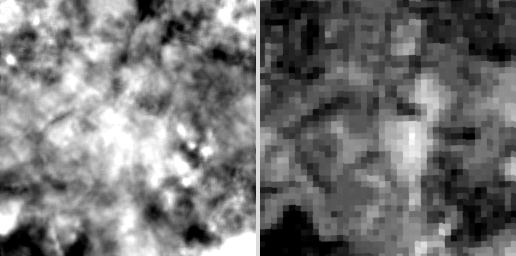
\includegraphics[width=\linewidth]{img/bands_gray/sample_000008_B01_panel.png}
        \caption{B1 (Aerosols, 443 nm)}
    \end{subfigure}\hfill
    \begin{subfigure}{0.48\textwidth}
        \centering
        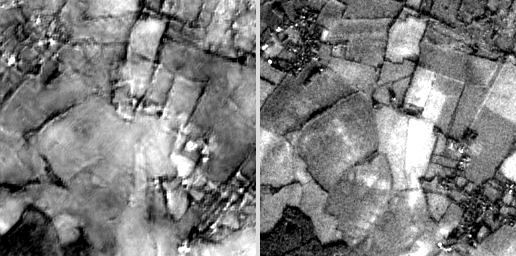
\includegraphics[width=\linewidth]{img/bands_gray/sample_000008_B02_panel.png}
        \caption{B2 (Blue, 490 nm)}
    \end{subfigure}

    % ---------- Row 2 ----------
    \vspace{0.5em}
    \begin{subfigure}{0.48\textwidth}
        \centering
        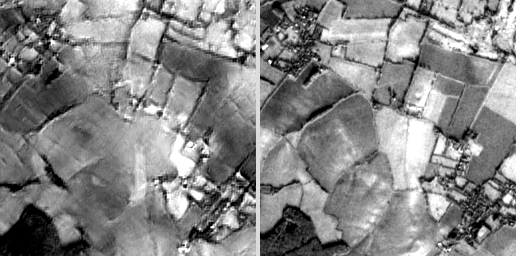
\includegraphics[width=\linewidth]{img/bands_gray/sample_000008_B03_panel.png}
        \caption{B3 (Green, 560 nm)}
    \end{subfigure}\hfill
    \begin{subfigure}{0.48\textwidth}
        \centering
        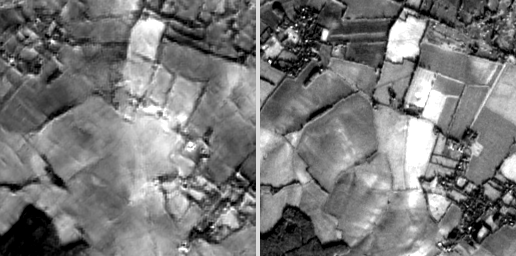
\includegraphics[width=\linewidth]{img/bands_gray/sample_000008_B04_panel.png}
        \caption{B4 (Red, 665 nm)}
    \end{subfigure}

    % ---------- Row 3 ----------
    \vspace{0.5em}
    \begin{subfigure}{0.48\textwidth}
        \centering
        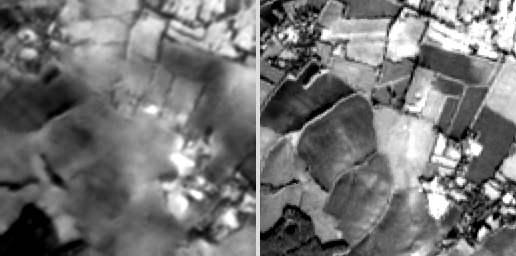
\includegraphics[width=\linewidth]{img/bands_gray/sample_000008_B05_panel.png}
        \caption{B5 (Red Edge, 705 nm)}
    \end{subfigure}\hfill
    \begin{subfigure}{0.48\textwidth}
        \centering
        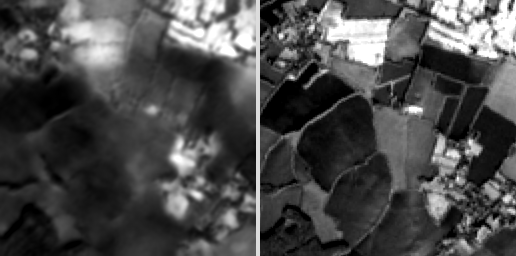
\includegraphics[width=\linewidth]{img/bands_gray/sample_000008_B06_panel.png}
        \caption{B6 (Red Edge, 740 nm)}
    \end{subfigure}

    \caption[Bandwise grayscale reconstructions (Bands 1–6)]%
    {Generated (left) and ground-truth (right) grayscale representations for Sentinel-2 Bands~1–6.}
    \label{fig:appendix_band_panels}
\end{figure}

\begin{figure}[p]
    \ContinuedFloat
    \centering
    \captionsetup[subfigure]{labelformat=empty}

    % ---------- Row 4 ----------
    \begin{subfigure}{0.48\textwidth}
        \centering
        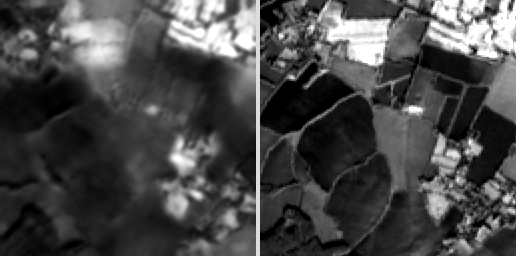
\includegraphics[width=\linewidth]{img/bands_gray/sample_000008_B07_panel.png}
        \caption{B7 (Red Edge, 783 nm)}
    \end{subfigure}\hfill
    \begin{subfigure}{0.48\textwidth}
        \centering
        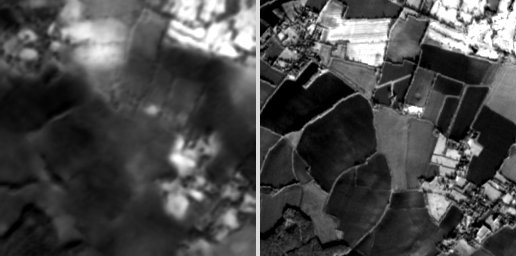
\includegraphics[width=\linewidth]{img/bands_gray/sample_000008_B08_panel.png}
        \caption{B8 (NIR, 842 nm)}
    \end{subfigure}

    % ---------- Row 5 ----------
    \vspace{0.5em}
    \begin{subfigure}{0.48\textwidth}
        \centering
        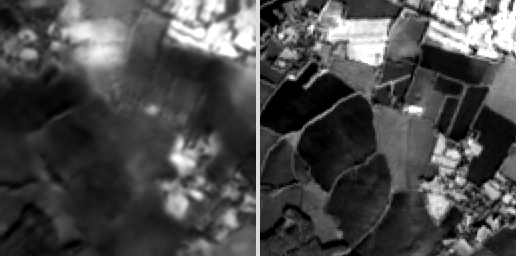
\includegraphics[width=\linewidth]{img/bands_gray/sample_000008_B09_panel.png}
        \caption{B8A (Red Edge, 865 nm)}
    \end{subfigure}\hfill
    \begin{subfigure}{0.48\textwidth}
        \centering
        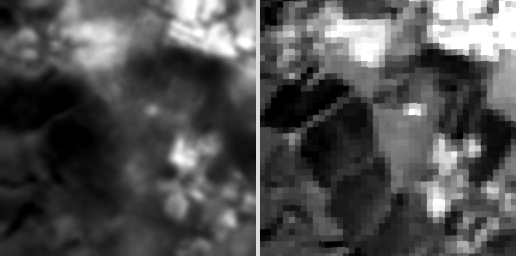
\includegraphics[width=\linewidth]{img/bands_gray/sample_000008_B10_panel.png}
        \caption{B9 (Water Vapour, 945 nm)}
    \end{subfigure}

    % ---------- Row 6 ----------
    \vspace{0.5em}
    \begin{subfigure}{0.48\textwidth}
        \centering
        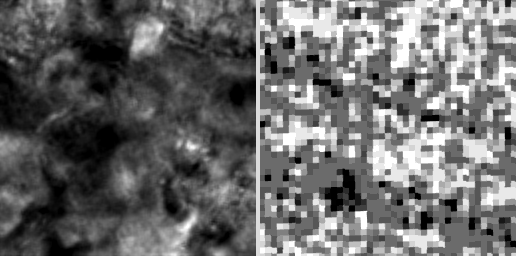
\includegraphics[width=\linewidth]{img/bands_gray/sample_000008_B11_panel.png}
        \caption{B10 (Cirrus, 1375 nm)}
    \end{subfigure}\hfill
    \begin{subfigure}{0.48\textwidth}
        \centering
        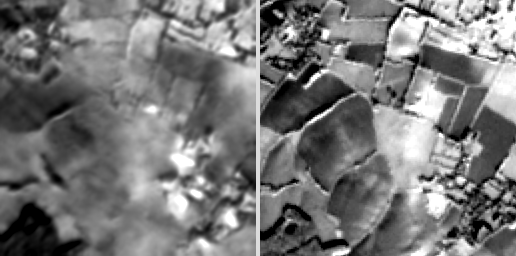
\includegraphics[width=\linewidth]{img/bands_gray/sample_000008_B12_panel.png}
        \caption{B11 (SWIR, 1610 nm)}
    \end{subfigure}

    % ---------- Row 7 ----------
    \vspace{0.5em}
    \begin{subfigure}{0.48\textwidth}
        \centering
        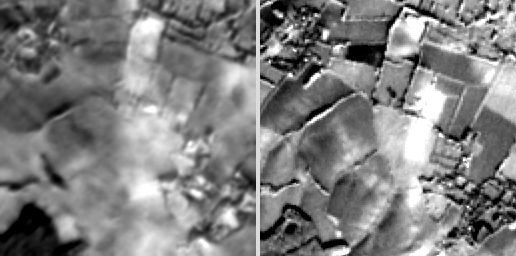
\includegraphics[width=\linewidth]{img/bands_gray/sample_000008_B13_panel.png}
        \caption{B12 (SWIR, 2190 nm)}
    \end{subfigure}

    \caption[Bandwise grayscale reconstructions (Bands 7–12)]%
    {Generated (left) and ground-truth (right) grayscale representations for Sentinel-2 Bands~7–12.}
\end{figure}

\chapter{Results Across Different Seasons}
\label{appendix:results_seasons}

% ---------------- FALL ----------------
\begin{table}[h!]
\centering
\caption[Quantitative results on the fall subset]{Quantitative performance of the model on the fall subset of the SEN12-MS dataset.}
\begin{tabular}{lcccc}
\toprule
\textbf{Season} & \textbf{SSIM} & \textbf{PSNR (dB)} & \textbf{LPIPS} & \textbf{SAM (°)} \\
\midrule
Fall & 0.788 & 22.40 & 0.269 & 13.67 \\
\bottomrule
\end{tabular}
\label{tab:fall_results}
\end{table}

% \vspace{1em} 

\begin{figure}[h!]
    \centering
    \setlength{\tabcolsep}{2pt}
    \renewcommand{\arraystretch}{1.0}
    \begin{tabular}{c *{3}{c}}
        
        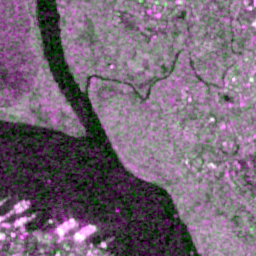
\includegraphics[width=0.25\textwidth]{img/seasons/fall/sample_000031_sar_pseudo.png} &
        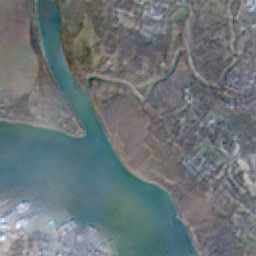
\includegraphics[width=0.25\textwidth]{img/seasons/fall/sample_000031_pred_rgb.png} &
        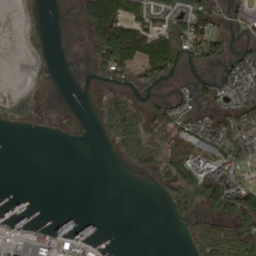
\includegraphics[width=0.25\textwidth]{img/seasons/fall/sample_000031_true_rgb.png} \\
        
        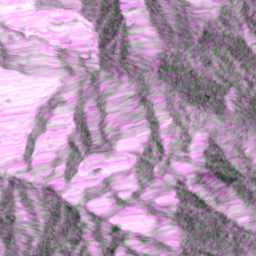
\includegraphics[width=0.25\textwidth]{img/seasons/fall/sample_000019_sar_pseudo.png} &
        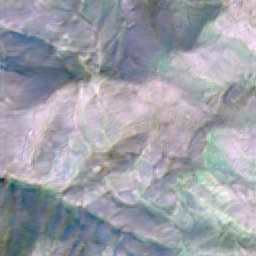
\includegraphics[width=0.25\textwidth]{img/seasons/fall/sample_000019_pred_rgb.png} &
        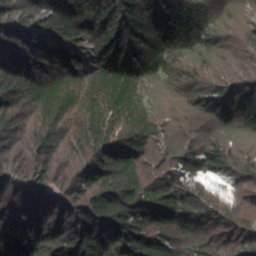
\includegraphics[width=0.25\textwidth]{img/seasons/fall/sample_000019_true_rgb.png} \\
        
        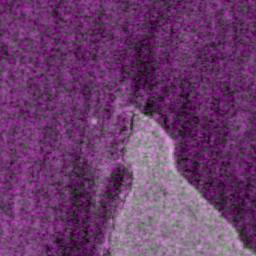
\includegraphics[width=0.25\textwidth]{img/seasons/fall/sample_000015_sar_pseudo.png} &
        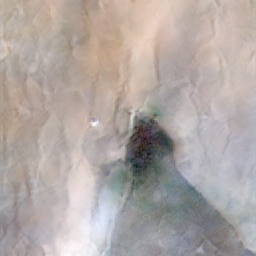
\includegraphics[width=0.25\textwidth]{img/seasons/fall/sample_000015_pred_rgb.png} &
        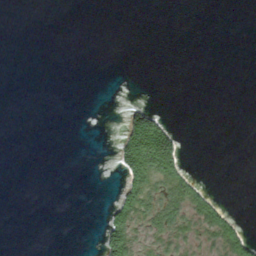
\includegraphics[width=0.25\textwidth]{img/seasons/fall/sample_000015_true_rgb.png} \\

    \end{tabular}
    \caption[Qualitative results on the fall subset]{%
    Representative SAR-to-optical translation result on the \textbf{fall} subset from the SEN12-MS dataset. 
    Columns: \textbf{(i)} SAR input (pseudo-RGB), 
    \textbf{(ii)} model-generated optical image, 
    \textbf{(iii)} ground-truth Sentinel-2 image.
    }
    \label{fig:appendix_fall}
\end{figure}

\newpage
% ---------------- SPRING ----------------
% \section{Spring Subset}
\vspace{2em} 

\begin{table}[h!]
\centering
\caption[Quantitative results on the spring subset]{Quantitative performance of the model on the spring subset of the SEN12-MS dataset.}
\begin{tabular}{lcccc}
\toprule
\textbf{Season} & \textbf{SSIM} & \textbf{PSNR (dB)} & \textbf{LPIPS} & \textbf{SAM (°)} \\
\midrule
Spring & 0.791 & 20.00 & 0.297 & 12.06 \\
\bottomrule
\end{tabular}
\label{tab:spring_results}
\end{table}
\vspace{2em} 


\begin{figure}[h!]
    \centering
    \setlength{\tabcolsep}{2pt}
    \renewcommand{\arraystretch}{1.0}
    \begin{tabular}{c *{3}{c}}
        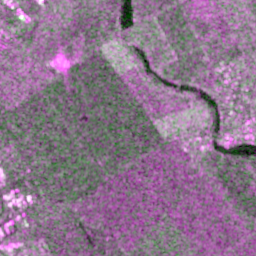
\includegraphics[width=0.25\textwidth]{img/seasons/spring/sample_000011_sar_pseudo.png} &
        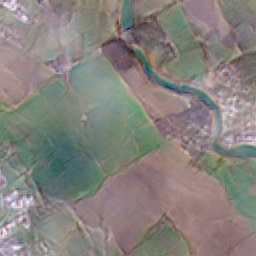
\includegraphics[width=0.25\textwidth]{img/seasons/spring/sample_000011_pred_rgb.png} &
        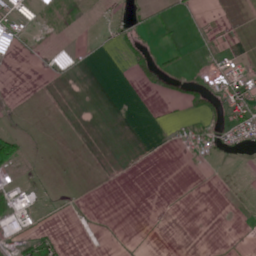
\includegraphics[width=0.25\textwidth]{img/seasons/spring/sample_000011_true_rgb.png} \\
        
        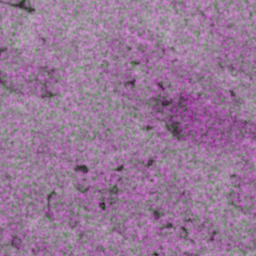
\includegraphics[width=0.25\textwidth]{img/seasons/spring/sample_000008_sar_pseudo.png} &
        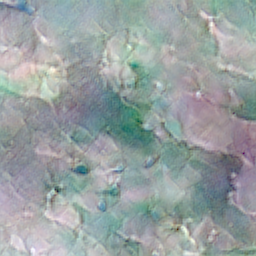
\includegraphics[width=0.25\textwidth]{img/seasons/spring/sample_000008_pred_rgb.png} &
        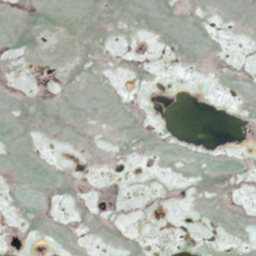
\includegraphics[width=0.25\textwidth]{img/seasons/spring/sample_000008_true_rgb.png} \\
        
        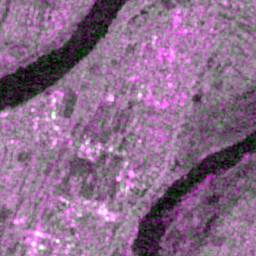
\includegraphics[width=0.25\textwidth]{img/seasons/spring/sample_000091_sar_pseudo.png} &
        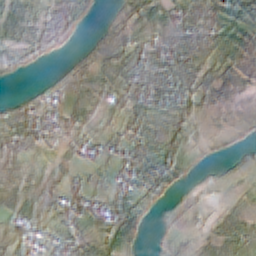
\includegraphics[width=0.25\textwidth]{img/seasons/spring/sample_000091_pred_rgb.png} &
        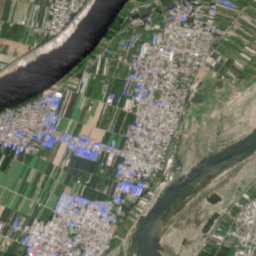
\includegraphics[width=0.25\textwidth]{img/seasons/spring/sample_000091_true_rgb.png} \\
    \end{tabular}
    \caption[Qualitative results on the spring subset]{%
    Representative SAR-to-optical translation result on the \textbf{spring} subset. 
    Columns: \textbf{(i)} SAR input (pseudo-RGB), 
    \textbf{(ii)} model-generated optical image, 
    \textbf{(iii)} ground-truth Sentinel-2 image.
    }
    \label{fig:appendix_spring}
\end{figure}


% ---------------- SUMMER ----------------
% \section{Summer Subset}
\newpage

\vspace{2em} 

\begin{table}[h!]
\centering
\caption[Quantitative results on the summer subset]{Quantitative performance of the model on the summer subset of the SEN12-MS dataset.}
\begin{tabular}{lcccc}
\toprule
\textbf{Season} & \textbf{SSIM} & \textbf{PSNR (dB)} & \textbf{LPIPS} & \textbf{SAM (°)} \\
\midrule
Summer & 0.800 & 22.79 & 0.268 & 12.43 \\
\bottomrule
\end{tabular}
\label{tab:summer_results}
\end{table}

\vspace{2em} 

\begin{figure}[h!]
    \centering
    \setlength{\tabcolsep}{2pt}
    \renewcommand{\arraystretch}{1.0}
    \begin{tabular}{c *{3}{c}}

        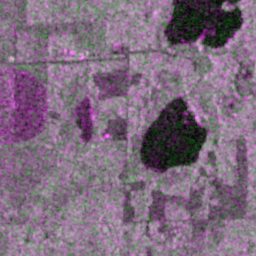
\includegraphics[width=0.25\textwidth]{img/seasons/summer/sample_000004_sar_pseudo.png} &
        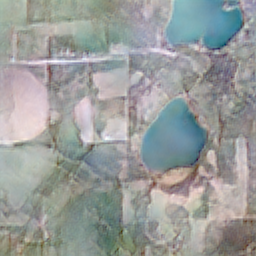
\includegraphics[width=0.25\textwidth]{img/seasons/summer/sample_000004_pred_rgb.png} &
        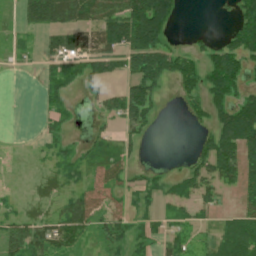
\includegraphics[width=0.25\textwidth]{img/seasons/summer/sample_000004_true_rgb.png} \\
        
        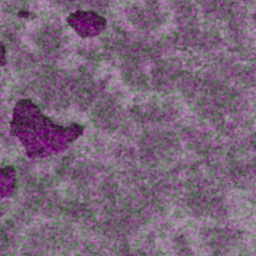
\includegraphics[width=0.25\textwidth]{img/seasons/summer/sample_000017_sar_pseudo.png} &
        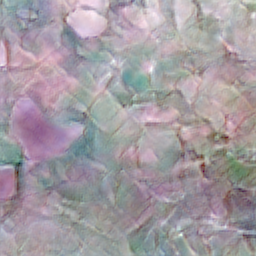
\includegraphics[width=0.25\textwidth]{img/seasons/summer/sample_000017_pred_rgb.png} &
        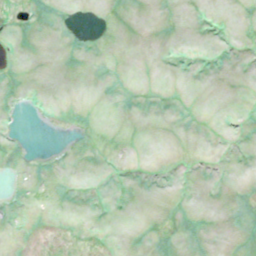
\includegraphics[width=0.25\textwidth]{img/seasons/summer/sample_000017_true_rgb.png} \\
        
        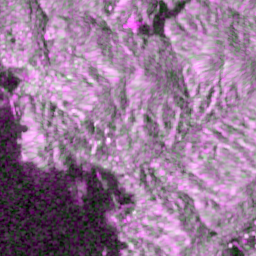
\includegraphics[width=0.25\textwidth]{img/seasons/summer/sample_000026_sar_pseudo.png} &
        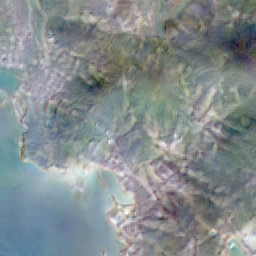
\includegraphics[width=0.25\textwidth]{img/seasons/summer/sample_000026_pred_rgb.png} &
        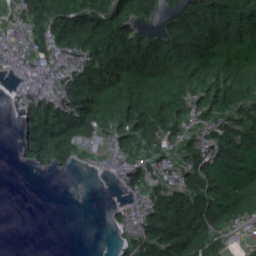
\includegraphics[width=0.25\textwidth]{img/seasons/summer/sample_000026_true_rgb.png} \\
    \end{tabular}
    \caption[Qualitative results on the summer subset]{%
    Representative SAR-to-optical translation result on the \textbf{summer} subset. 
    Columns: \textbf{(i)} SAR input (pseudo-RGB), 
    \textbf{(ii)} model-generated optical image, 
    \textbf{(iii)} ground-truth Sentinel-2 image.
    }
    \label{fig:appendix_summer}
\end{figure}

